\begin{frame}
  \begin{center}
    {\color{Maroon}\Huge Tackling New Languages}
  \end{center}
\end{frame}

\begin{frame}{Tackling New Languages}{Outline}
  \begin{enumerate}
  \item IARPA Babel
  \item Audio Keyword Search
  \item What Language Characteristics Matter?
  \item A Recipe for a New Language
    \begin{itemize}
    \item Pronunciations
    \item Flat-start Initialization
    \item Multilingual Features
    \item Web Text
    \end{itemize}
  \end{enumerate}
\end{frame}

\begin{frame}{The IARPA Babel Program}{}
  \Large{``\ldots to \alert{rapidly develop} speech recognition
    capability for keyword search in a previously unstudied
    language, working with speech recorded in a variety of
    conditions with limited amounts of transcription.''}\par
\end{frame}

\begin{frame}{Rapid Development}{Time allowed for surprise language model building}
  \centering
  \begin{tabular}{@{}cl@{}} \toprule
    {\bf Period} & \multicolumn{1}{c}{\bf Time} \\ \midrule
    1 & 4 weeks \\
    2 & 3 weeks \\
    3 & 2 weeks \\
    4 & 1 week  \\ \bottomrule
  \end{tabular}
\end{frame}

\begin{frame}{The IARPA Babel Program}{}
  \Large{``\ldots to rapidly develop speech recognition
    capability for keyword search in a \alert{previously unstudied
      language}, working with speech recorded in a variety of
    conditions with limited amounts of transcription.''}\par
\end{frame}

\begin{frame}{Babel Languages}{}
  \begin{center}
  \begin{tabular}{@{}llll@{}} \toprule
    \multicolumn{1}{c}{\bf Period 1} & \multicolumn{1}{c}{\bf Period 2} & \multicolumn{1}{c}{\bf Period 3} & \multicolumn{1}{c}{\bf Period 4} \\ \midrule
    Cantonese  & Assamese       & Kurmanji Kurdish & Pashto \\
    Pashto     & Bengali        & Tok Pisin        & Guaran\'{i} \\
    Turkish    & Haitian Creole & Cebuano          & Igbo \\
    Tagalog    & Lao            & Kazakh           & Amharic \\
    Vietnamese & Zulu           & Telugu           & Mongolian \\
               & Tamil          & Lithuanian       & Javanese \\
               &                & Swahili          & Dholuo \\
               &                &                  & Georgian \\ \bottomrule
  \end{tabular}
  \end{center}
  \vfill
  \nb{These will be available from the LDC at \$US 25.00 per language for non-members.}
\end{frame}

\begin{frame}{The IARPA Babel Program}{}
  \Large{``\ldots to rapidly develop speech recognition
    capability for keyword search in a previously unstudied
    language, working with speech recorded in a variety of
    conditions with \alert{limited amounts of transcription}.''}\par
\end{frame}

\begin{frame}{Limited resources}{Hours of transcribed training data}
  \settowidth{\colA}{100}
  \begin{center}
    \begin{tabular}{@{}cc@{}} \toprule
      {\bf Period} & {\bf Hours} \\ \midrule
      1 & 100 \\
      2 & \aln{\colA}{r}{10} \\
      3 & \aln{\colA}{r}{3}  \\
      4 & \aln{\colA}{r}{40} \\ \bottomrule
    \end{tabular}
  \end{center}
  \vfill
  \nb{In Periods 3 and 4, no phonetic lexicons.}
\end{frame}

\begin{frame}{The IARPA Babel Program}{}
  \Large{``\ldots to rapidly develop speech recognition
    capability for \alert{keyword search} in a previously unstudied
    language, working with speech recorded in a variety of
    conditions with limited amounts of transcription.''}\par
\end{frame}

\begin{frame}{What is keyword search, and why focus on it?}{}
  {\bf Detection task}: given
    \begin{itemize}
    \item a word or short phrase and
    \item a collection of speech data,
    \end{itemize}
    does it occur, and if so where does it occur, and how confident are you?
    \vfill
    We can build practical keyword search from
    \alert{unreliable} speech recognition.
\end{frame}

\begin{frame}{Weighted Finite-State Acceptors}{}
  A \alert{weighted finite-state acceptor} compactly represents a set
  of strings, with a score assigned to each string.
  \vfill
  Formally, a WFSA comprises
  \begin{description}
  \item[states] some of which are start states, end states, or both;
    and
  \item[edges] between states, labeled with symbols from a finite
    alphabet and scores.
  \end{description}
\end{frame}

\begin{frame}{An Example}{}
  \begin{center}
    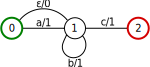
\includegraphics[width=72mm]{figures/WFSA}
  \end{center}
  \vfill
  Represents {\tt a?b*c} and the score of each string is its length.
\end{frame}

\begin{frame}{Weighted Finite-State Transducers}{}
  A \alert{weighted finite-state transducer} compactly represents a
  relation between two sets of strings, with a score assigned to each
  output string.
  \vfill
  Formally, a WFST comprises
  \begin{description}
  \item[states] some of which are start states, end states, or both;
    and
  \item[edges] between states, labeled with input symbols from a
    finite alphabet, output samples from a (potentially different)
    finite alphabet, and scores.
  \end{description}
\end{frame}

\begin{frame}{An Example}{}
  \begin{center}
    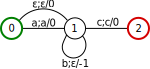
\includegraphics[width=72mm]{figures/WFST}
  \end{center}
  \vfill
  Maps strings in {\tt a?b*c} to {\tt a?c} by deleting {\tt b} symbols
  and the score of each string the change in its length.
\end{frame}

\begin{frame}{Composition}{}
  \begin{center}
    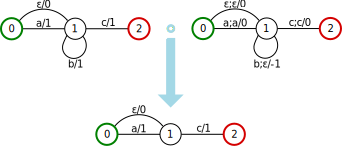
\includegraphics[width=96mm]{figures/Composition}
  \end{center}
  \vfill
  Given WFSA $\mathcal{S}$ and WFST $\mathcal{T}$, their composition
  $\mathcal{T} \circ \mathcal{S}$ is a WFSA that represents the set of
  strings (and corresponding scores) obtained by applying
  $\mathcal{T}$ to the set of strings represented by $\mathcal{S}$.
\end{frame}

\begin{frame}{Roadmap for WFST-based keyword search}{}
  \begin{enumerate}
  \item Form a WFST index representing a relation between
    \begin{description}
      \item[inputs] all high-probability strings of words or phones in
        the collection,
      \item[outputs] times of occurrence of the words or phones, and
      \item[scores] probabilities of the strings;
    \end{description}
    \item Form a WFSA representing a query; then
    \item \alert{compose} the query WFSA with the index WFST to
      perform the search.
  \end{enumerate}
\end{frame}

%% WFST search:  index generation (token and phonetic)
\begin{frame}{Building an index}{1. Generate a lattice for each segment in the collection.}
  \begin{center}
    
\includegraphics[width=36mm]{figures/lattice}
  \end{center}
  \begin{overlayarea}{\textwidth}{24mm}
    \begin{columns}[t]
      \column{54mm}
      \onslide<1>{
        \centerline{\bf Lattice}
        \begin{description}
        \item[Nodes] times
        \item[Edges] words (or phones) and posterior probabilities
        \end{description}
      }
      \column{54mm}
      \onslide<2>{
        \centerline{\bf Transducer}
        \begin{description}
        \item[Inputs] words (or phones)
        \item[Outputs] times
        \item[Scores] negative log-posteriors
        \end{description}
      }
    \end{columns}
  \end{overlayarea}
\end{frame}

\begin{frame}{Building an index}{2. Produce the factor automaton for each segment.}
  \begin{center}
    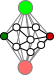
\includegraphics[width=36mm]{figures/factor}
    \end{center}
  \vfill
  Added edges have $\epsilon$ inputs, $\epsilon$ outputs, and no costs.
\end{frame}

\begin{frame}{Building an index}{3. Connect all the factor automata in parallel.}
  \begin{center}
    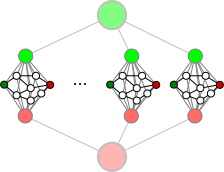
\includegraphics[width=66mm]{figures/index}
    \end{center}
  \vfill
  Added edges from start have $\epsilon$ inputs, segment ID outputs, and no costs.
  Added edges to end have $\epsilon$ inputs, $\epsilon$ outputs, and no costs.
\end{frame}

\begin{frame}{Building a query}{}
  In-vocabulary queries are simple:
  \begin{enumerate}
  \item use a word-based WFST index, and
  \item represent queries as word-level linear-chain WFSAs.
  \end{enumerate}
  \vfill
  Queries containing \alert{out-of-vocabulary} words are more challenging.
\end{frame}

\begin{frame}{Handling out-of-vocabulary queries}{}
  \begin{enumerate}
  \item represent queries as phone-level linear-chain WFSAs,
  \item compose the WFSAs with a WFST \alert{confusability} model,
  \item prune the resulting WFSAs, and
  \item {\bf if a word-based index is used}, compose the query WFSAs
    with a WFST that maps phone sequences back to words.
  \end{enumerate}
  \vfill
  The confusability model is created by running speech recognition on
  the training data and counting co-occurrences of reference and
  hypothesized phones.
  \vfill
  \nb{This is a form of query expansion, which is well
    studied in the information retrieval literature.}
\end{frame}

\begin{frame}{How do we measure keyword search performance?}
  {Actual Term-Weighted Value (ATWV)}
  \begin{equation*}
    \text{ATWV}(\theta) = \frac{1}{N}\sum_{q}
    \left[
      \frac{N_{\text{hit}}(q;\theta)}{N_{\text{true}}(q)} -
      \beta \frac{N_{\text{FA}}(q;\theta)}{T - N_{\text{true}}(q)}
      \right]
  \end{equation*}
  \begin{itemize}
  \item There are $N$ test queries indexed by $q$,
  \item $\theta$ is a decision threshold,
  \item $N_{\text{hit}}(q;\theta)$ is the number of correct detections and
  \item $N_{\text{FA}}(q;\theta)$ is the number of false alarms for
    query $q$ at decision threshold $\theta$, 
  \item $N_{\text{true}}(q)$ is the number of occurrences of query $q$
    in the test audio,
  \item $T$ is the duration of the test audio in seconds, and
  \item $\beta = 999.9$ is a weight on the penalty for false alarms.
  \end{itemize}
\end{frame}

\begin{frame}{Breaking it down}{}
  \begin{overlayarea}{\textwidth}{56mm}
  \only<1>{
  \begin{equation*}
    \text{ATWV}(\theta) = \frac{1}{N}\sum_{q}
    \left[
      {\color{red}\frac{N_{\text{hit}}(q;\theta)}{N_{\text{true}}(q)}} -
      \beta \frac{N_{\text{FA}}(q;\theta)}{T - N_{\text{true}}(q)}
      \right]
  \end{equation*}
  }
  \only<2>{
  \begin{equation*}
    \text{ATWV}(\theta) = \frac{1}{N}\sum_{q}
    \left[
      \frac{N_{\text{hit}}(q;\theta)}{N_{\text{true}}(q)} -
      {\color{red}\beta \frac{N_{\text{FA}}(q;\theta)}{T - N_{\text{true}}(q)}}
      \right]
  \end{equation*}
  }
  \only<3>{
  \begin{equation*}
    \text{ATWV}(\theta) = \frac{1}{N}\sum_{q}
    \left[
      \frac{N_{\text{hit}}(q;\theta)}{N_{\text{true}}(q)} -
      \beta \frac{N_{\text{FA}}(q;\theta)}{T - N_{\text{true}}(q)}
      \right]
  \end{equation*}
  }
  \vspace*{8mm}
  \begin{itemize}
  \item<1-> Hits earn a reward of $\frac{1}{N \cdot N_{\text{true}}(q)}$, so
    rare terms are more valuable.
  \item<2-> False alarms incur a constant loss of approximately
    $\frac{\beta}{N \cdot T}$ (because $T \gg N_{\text{true}}(q)$ for all $q$).
  \item<3-> Perfect performance scores $\text{ATWV} = 1.0$, while
    empty output scores $\text{ATWV} = 0.0$.  $\text{ATWV} < 0.0$
    means you have too many false alarms!
  \end{itemize}
  \end{overlayarea}
  \vfill
  \nb{Score normalization is important under the ATWV metric.  For
    more details on this issue, please see \cite{Wang2014}.}
\end{frame}

\begin{frame}{Babel Languages}{}
  \begin{center}
    \begin{tabular}{@{}llll@{}} \toprule
      \multicolumn{1}{c}{\bf Period 1} & \multicolumn{1}{c}{\bf Period 2} & \multicolumn{1}{c}{\bf Period 3} & \multicolumn{1}{c}{\bf Period 4} \\ \midrule
      Cantonese  & Assamese       & Kurmanji Kurdish & Pashto \\
      Pashto     & Bengali        & Tok Pisin        & Guaran\'{i} \\
      Turkish    & Haitian Creole & Cebuano          & Igbo \\
      Tagalog    & Lao            & Kazakh           & Amharic \\
      Vietnamese & Zulu           & Telugu           & Mongolian \\
                 & Tamil          & Lithuanian       & Javanese \\
                 &                & Swahili          & Dholuo \\
                 &                &                  & Georgian \\ \bottomrule
    \end{tabular}
  \end{center}
\end{frame}

\begin{frame}{What language characteristics matter?}{}
  \begin{enumerate}
  \item Morphology
  \item Writing system
  \item Tonal languages
  \item Amount of available training data
  \end{enumerate}
\end{frame}

%% Morphology and vocabulary growth
\begin{frame}{Morphology}{}
  The morphology of a language refers to the structure of its words.
  Specifically, are words atomic, or are they composed from meaningful
  parts?
  \vfill
  {\color{DarkerBlue}\bf English example} \\
  re+ +do+ +er --- one who is performing some action again
  \vfill
  Languages with \alert{agglutinative} morphology have large
  inventories of words formed by the composition of smaller units
  (morphs).
  \vfill
  One way to characterize this is through vocabulary growth.
\end{frame}

\begin{frame}{Vocabulary Growth for Babel Languages}{}
  \begin{center}
    \includegraphics[width=108mm]{figures/vocGrowth}
  \end{center}
\end{frame}

\begin{frame}{Mitigating Rapid Vocabulary Growth}{}
  Out-of-vocabulary words are more likely to occur in test data for
  languages with rapid vocabulary growth, which will degrade speech
  recognition and keyword search performance.
  \vfill
  Two ways to reduce the impact:
  \begin{description}[morph models]
    \item[morph models] base the vocabulary on morphs instead of
      words, and
    \item[web text] expand the vocabulary by collecting text from the
      web.
  \end{description}
\end{frame}

\begin{frame}{Morph Models}{}
  Recipe:
  \begin{enumerate}
  \item Segment the training text into morph-like units using
    Morfessor~\cite{Morfessor} or some other tool.
  \item Generate a pronunciation lexicon for the morphs.
  \item Train a language model on the segmented training text.
  \end{enumerate}
  \vfill
  Task-specific considerations:
  \begin{description}
  \item[ASR]
    \begin{itemize}
    \item Recomposing morphs into words is challenging.
    \end{itemize}
  \item[KWS]
    \begin{itemize}
      \item Need to decompose queries into morphs.
      \item Best results obtained by doing word and morph search, and
        fusing the results.
    \end{itemize}
  \end{description}
\end{frame}

\begin{frame}{Keyword Search Results with Morph Models}{}
  \begin{columns}[c]
    \column{68mm}
    \centering
    \begin{tabular}{@{}lcc@{}} \toprule
      & {\bf Word} & {\bf Word+Morph} \\
      {\bf Language} & {\bf MTWV} & {\bf MTWV} \\ \midrule
      Zulu     & 0.1817 & 0.2305 \\
      Assamese & 0.2643 & 0.2797 \\ \bottomrule
    \end{tabular}
    \column{40mm}
    \centering{\includegraphics[width=40mm]{figures/vocGrowthThumb}}
  \end{columns}
  \vfill
  \nb{Maximum Term-Weighted Value (MTWV) is ATWV with an oracle
    decision threshold.}
\end{frame}

\begin{frame}{Web Text}{}
  General considerations:
  \begin{itemize}
  \item How much web presence does the language have?
    \begin{itemize}
    \item Swahili: plenty
    \item Dholuo: sparse
    \end{itemize}
  \item How easy is it to generate queries returning the target language?
    \begin{itemize}
    \item Amharic has its own Unicode range, so it is easy.
    \item Tagalog contains many English and Spanish loanwords, so it
      is difficult.
    \end{itemize}
  \item Normalization is a must!
  \end{itemize}
\end{frame}

\begin{frame}{Web Text}{}
  Task-specific considerations:
  \begin{description}
  \item[ASR] Improvements may be small due to genre mismatch (LM is important).
  \item[KWS] Better vocabulary coverage improves performance (LM is not important).
  \end{description}
\end{frame}

\begin{frame}{Impact of Web Text}{}
  \centering
  \begin{tabular}{@{}lcd{5.1}d{3.1}cc@{}} \toprule
    & & \multicolumn{1}{c}{\bf Train} & \multicolumn{1}{c}{\bf Voc.} &               &            \\
    {\bf Language} & {\bf Web?} & \multicolumn{1}{c}{\bf size} & \multicolumn{1}{c}{\bf size} & {\bf \% WER} & {\bf MTWV} \\ \midrule


    Igbo        & N &    45.3 & 16.5 & 66.5 & 0.2387 \\
                & Y &   707.  & 19.3 & 66.5 & 0.2389 \\ \midrule
    Guaran\'{i} & N &    46.8 & 26.3 & 53.5 & 0.4562 \\
                & Y &   437.  & 36.8 & 53.5 & 0.4665 \\ \midrule
    Mongolian   & N &    51.2 & 23.6 & 61.1 & 0.3497 \\
                & Y & 55300.  & 217. & 60.4 & 0.3849 \\ \bottomrule
  \end{tabular}
  \vfill
  \raggedright
  Word counts are in thousands.
\end{frame}

%% \begin{frame}{Impact of Web Text}{}
%%   \centering
%%   \begin{tabular}{@{}lcd{3.1}d{2.1}cc@{}} \toprule
%%     & & \multicolumn{1}{c}{\bf Voc.}     & \multicolumn{1}{c}{\bf \% OOV}  &              &            \\
%%     {\bf Language} & {\bf Web?} & \multicolumn{1}{c}{\bf size (K)} & \multicolumn{1}{c}{\bf queries} & {\bf \% WER} & {\bf MTWV} \\ \midrule
%%     Igbo        & N & 16.5 & 11.9 & 66.5 & 0.2387 \\
%%                 & Y & 19.3 & 11.6 & 66.5 & 0.2389 \\ \midrule
%%     Guaran\'{i} & N & 26.3 & 13.8 & 53.5 & 0.4562 \\
%%                 & Y & 36.8 & 12.9 & 53.5 & 0.4665 \\ \midrule
%%     Mongolian   & N & 23.6 & 12.2 & 61.1 & 0.3497 \\
%%                 & Y & 217. &  3.8 & 60.4 & 0.3849 \\ \bottomrule
%%   \end{tabular}
%% \end{frame}

%% Writing system ... only matters if you don't have a phonetic
%% pronunciation lexicon
%% - Ideographic
%% - Alphabet
%% - Abjad
%% - Abugida
%% Ideographic languages require a character-to-pronunciation
%% lexicon, while in many cases the other writing systems may be
%% handled with simple rule-based spelling-to-sound conversion.

%% Tonal languages
%% If so, must represent pitch
%% explicit - e.g. FFV features
%% implicit - e.g. high-resolution Mel spectral features in NN
%% give results for Lao

%% Amount of available training data
%%   multilingual feature front-ends
%%   multilingual AMs
%%   Data augmentation
%%   Semi-supervised training

%% A Recipe for a New Language (do a VLLP and a recent FLP?)
%% Pronunciations
%% Flat-start Initialization
%% Multilingual Features
%% Web Text

%% \begin{frame}{}{}
%% \end{frame}
